%===============================================================================
% LaTeX sjabloon voor de bachelorproef toegepaste informatica aan HOGENT
% Meer info op https://github.com/HoGentTIN/latex-hogent-report
%===============================================================================

\documentclass[dutch,dit,thesis]{hogentreport}

% TODO:
% - If necessary, replace the option `dit`' with your own department!
%   Valid entries are dbo, dbt, dgz, dit, dlo, dog, dsa, soa
% - If you write your thesis in English (remark: only possible after getting
%   explicit approval!), remove the option "dutch," or replace with "english".

\usepackage{lipsum} % For blind text, can be removed after adding actual content

%% Pictures to include in the text can be put in the graphics/ folder
\graphicspath{{../graphics/}}

%% For source code highlighting, requires pygments to be installed
%% Compile with the -shell-escape flag!
%% \usepackage[chapter]{minted}
%% If you compile with the make_thesis.{bat,sh} script, use the following
%% import instead:
\usepackage[chapter,outputdir=../output]{minted}
\usemintedstyle{solarized-light}

%% Formatting for minted environments.
\setminted{%
    autogobble,
    frame=lines,
    breaklines,
    linenos,
    tabsize=4
}

%% Ensure the list of listings is in the table of contents
\renewcommand\listoflistingscaption{%
    \IfLanguageName{dutch}{Lijst van codefragmenten}{List of listings}
}
\renewcommand\listingscaption{%
    \IfLanguageName{dutch}{Codefragment}{Listing}
}
\renewcommand*\listoflistings{%
    \cleardoublepage\phantomsection\addcontentsline{toc}{chapter}{\listoflistingscaption}%
    \listof{listing}{\listoflistingscaption}%
}

% Other packages not already included can be imported here

%%---------- Document metadata -------------------------------------------------
% TODO: Replace this with your own information
\author{Ernst Aarden}
\supervisor{Dhr. F. Van Houte}
\cosupervisor{Mevr. S. Beeckman}
\title[Optionele ondertitel]%
    {Titel van de bachelorproef}
\academicyear{\advance\year by -1 \the\year--\advance\year by 1 \the\year}
\examperiod{1}
\degreesought{\IfLanguageName{dutch}{Professionele bachelor in de toegepaste informatica}{Bachelor of applied computer science}}
\partialthesis{false} %% To display 'in partial fulfilment'
%\institution{Internshipcompany BVBA.}

%% Add global exceptions to the hyphenation here
\hyphenation{back-slash}

%% The bibliography (style and settings are  found in hogentthesis.cls)
\addbibresource{bachproef.bib}            %% Bibliography file
\addbibresource{../voorstel/voorstel.bib} %% Bibliography research proposal
\defbibheading{bibempty}{}

%% Prevent empty pages for right-handed chapter starts in twoside mode
\renewcommand{\cleardoublepage}{\clearpage}

\renewcommand{\arraystretch}{1.2}

%% Content starts here.
\begin{document}

%---------- Front matter -------------------------------------------------------

\frontmatter

\hypersetup{pageanchor=false} %% Disable page numbering references
%% Render a Dutch outer title page if the main language is English
\IfLanguageName{english}{%
    %% If necessary, information can be changed here
    \degreesought{Professionele Bachelor toegepaste informatica}%
    \begin{otherlanguage}{dutch}%
       \maketitle%
    \end{otherlanguage}%
}{}

%% Generates title page content
\maketitle
\hypersetup{pageanchor=true}

%%=============================================================================
%% Voorwoord
%%=============================================================================

\chapter*{\IfLanguageName{dutch}{Woord vooraf}{Preface}}%
\label{ch:voorwoord}

%% TODO:
%% Het voorwoord is het enige deel van de bachelorproef waar je vanuit je
%% eigen standpunt (``ik-vorm'') mag schrijven. Je kan hier bv. motiveren
%% waarom jij het onderwerp wil bespreken.
%% Vergeet ook niet te bedanken wie je geholpen/gesteund/... heeft

\lipsum[1-2]
%%=============================================================================
%% Samenvatting
%%=============================================================================

% TODO: De "abstract" of samenvatting is een kernachtige (~ 1 blz. voor een
% thesis) synthese van het document.
%
% Een goede abstract biedt een kernachtig antwoord op volgende vragen:
%
% 1. Waarover gaat de bachelorproef?
% 2. Waarom heb je er over geschreven?
% 3. Hoe heb je het onderzoek uitgevoerd?
% 4. Wat waren de resultaten? Wat blijkt uit je onderzoek?
% 5. Wat betekenen je resultaten? Wat is de relevantie voor het werkveld?
%
% Daarom bestaat een abstract uit volgende componenten:
%
% - inleiding + kaderen thema
% - probleemstelling
% - (centrale) onderzoeksvraag
% - onderzoeksdoelstelling
% - methodologie
% - resultaten (beperk tot de belangrijkste, relevant voor de onderzoeksvraag)
% - conclusies, aanbevelingen, beperkingen
%
% LET OP! Een samenvatting is GEEN voorwoord!

%%---------- Nederlandse samenvatting -----------------------------------------
%
% TODO: Als je je bachelorproef in het Engels schrijft, moet je eerst een
% Nederlandse samenvatting invoegen. Haal daarvoor onderstaande code uit
% commentaar.
% Wie zijn bachelorproef in het Nederlands schrijft, kan dit negeren, de inhoud
% wordt niet in het document ingevoegd.

\IfLanguageName{english}{%
\selectlanguage{dutch}
\chapter*{Samenvatting}
\lipsum[1-4]
\selectlanguage{english}
}{}

%%---------- Samenvatting -----------------------------------------------------
% De samenvatting in de hoofdtaal van het document

\chapter*{\IfLanguageName{dutch}{Samenvatting}{Abstract}}

\lipsum[1-4]


%---------- Inhoud, lijst figuren, ... -----------------------------------------

\tableofcontents

% In a list of figures, the complete caption will be included. To prevent this,
% ALWAYS add a short description in the caption!
%
%  \caption[short description]{elaborate description}
%
% If you do, only the short description will be used in the list of figures

\listoffigures

% If you included tables and/or source code listings, uncomment the appropriate
% lines.
\listoftables

\listoflistings

% Als je een lijst van afkortingen of termen wil toevoegen, dan hoort die
% hier thuis. Gebruik bijvoorbeeld de ``glossaries'' package.
% https://www.overleaf.com/learn/latex/Glossaries

%---------- Kern ---------------------------------------------------------------

\mainmatter{}

% De eerste hoofdstukken van een bachelorproef zijn meestal een inleiding op
% het onderwerp, literatuurstudie en verantwoording methodologie.
% Aarzel niet om een meer beschrijvende titel aan deze hoofdstukken te geven of
% om bijvoorbeeld de inleiding en/of stand van zaken over meerdere hoofdstukken
% te verspreiden!

%%=============================================================================
%% Inleiding
%%=============================================================================

\chapter{\IfLanguageName{dutch}{Inleiding}{Introduction}}%
\label{ch:inleiding}

% De inleiding moet de lezer net genoeg informatie verschaffen om het onderwerp te begrijpen en in te zien waarom de onderzoeksvraag de moeite waard is om te onderzoeken. In de inleiding ga je literatuurverwijzingen beperken, zodat de tekst vlot leesbaar blijft. Je kan de inleiding verder onderverdelen in secties als dit de tekst verduidelijkt. Zaken die aan bod kunnen komen in de inleiding~\autocite{Pollefliet2011}:

% \begin{itemize}
%   \item context, achtergrond
%   \item afbakenen van het onderwerp
%   \item verantwoording van het onderwerp, methodologie
%   \item probleemstelling
%   \item onderzoeksdoelstelling
%   \item onderzoeksvraag
%   \item \ldots
% \end{itemize}

In een tijdperk waarin digitale transformatie en hybride cloudomgevingen de norm zijn geworden, is een geïntegreerde aanpak van netwerk en beveiliging centraal komen te staan voor softwarebedrijven. 
Traditionele netwerkmodellen, gebaseerd op perimeterbescherming via firewalls en VPNs, volstaan niet langer in een wereld van directe cloud-toegang, telewerken en verspreide applicaties. 

\vspace{2ex}

SASE (Secure Access Service Edge) biedt een geïntegreerd framework dat netwerk- en beveiligingsfuncties combineert in één cloudgebaseerd servicemodel. Voor softwarebedrijven met gevoelige klantdata, is deze aanpak essentieel om compliance te waarborgen en vertrouwen te behouden.

\vspace{2ex}

In dit onderzoek wordt de implementatie van een SASE (Secure Access Service Edge) oplossing, met de focus op Netskope, onderzocht.
\section{\IfLanguageName{dutch}{Probleemstelling}{Problem Statement}}%
\label{sec:probleemstelling}

% Uit je probleemstelling moet duidelijk zijn dat je onderzoek een meerwaarde heeft voor een concrete doelgroep. De doelgroep moet goed gedefinieerd en afgelijnd zijn. Doelgroepen als ``bedrijven,'' ``KMO's'', systeembeheerders, enz.~zijn nog te vaag. Als je een lijstje kan maken van de personen/organisaties die een meerwaarde zullen vinden in deze bachelorproef (dit is eigenlijk je steekproefkader), dan is dat een indicatie dat de doelgroep goed gedefinieerd is. Dit kan een enkel bedrijf zijn of zelfs één persoon (je co-promotor/opdrachtgever).

Het onderzochte softwarebedrijf is gespecialiseerd in digitale producten. Het kampt met toenemende uitdagingen rond netwerktoegang en security in zijn hybride cloudinfrastructuur.

\vspace{2ex}

\textbf{Specifieke pijnpunten zijn:}

\begin{itemize}
  \item User \& Device: Authenticatie en autorisatie van gebruikers en apparaten.
	\item Application \& Workload: Applicatie-specifieke toegangscontrole en monitoring.
  \item Data: Databescherming en classificatie
  \item Connectivity: veilige verbinding tussen cloud- en at home-omgevingen.
\end{itemize}

Om deze uitdagingen aan te pakken, heeft het bedrijf gekozen voor het Netskopeplatform om een SASE-architectuur te implementeren. Deze keuze vereist echter een gedetailleerd inzicht in de technische mogelijkheden van Netskope en een op maat gemaakte implementatiestrategie die zowel netwerk- als beveiligingsaspecten integreert.

\section{\IfLanguageName{dutch}{Onderzoeksvraag}{Research question}}%
\label{sec:onderzoeksvraag}

% Wees zo concreet mogelijk bij het formuleren van je onderzoeksvraag. Een onderzoeksvraag is trouwens iets waar nog niemand op dit moment een antwoord heeft (voor zover je kan nagaan). Het opzoeken van bestaande informatie (bv. ``welke tools bestaan er voor deze toepassing?'') is dus geen onderzoeksvraag. Je kan de onderzoeksvraag verder specifiëren in deelvragen. Bv.~als je onderzoek gaat over performantiemetingen, dan 

Hoe kan een SASE-architectuur worden geïmplementeerd binnen de hybride cloudomgeving van een softwarebedrijf gebruikmakend van het Netskope platform?

\vspace{2ex}

Deze vraag wordt opgesplitst in probleem- en oplossingsdomein:

\textbf{Probleemdomein}
\begin{itemize}
  \item Welke netwerk- en security-uitdagingen in de huidige infrastructuur kunnen worden aangepakt via Netskope's SASE-functionaliteiten?
  \item Welke tekortkomingen in de huidige perimeterbeveiliging vereisen een Zero Trust-aanpak?
\end{itemize}

\vspace{2ex}

\textbf{Oplossingsdomein}
\begin{itemize}
  \item Welke Netskope-componenten zijn nodig voor een succesvolle implementatie?
  \item Hoe kan Netskope geoptimaliseerd worden voor een hybride omgeving, inclusief integratie met bestaande systemen?
\end{itemize}

\vspace{2ex}

\textbf{Deelvragen}
\begin{itemize}
  \item Wat is de huidige situatie van het bedrijf op vlak van security en welke risico’s zijn er?
  \item Welke Netskope-functionaliteiten zijn relevant voor de implementatie van Zero Trust?
  \item Hoe kan Netskope geïntegreerd worden met bestaande systemen en processen?
  \item Hoe kan de implementatie van Netskope gevalideerd worden?
\end{itemize}

\section{\IfLanguageName{dutch}{Onderzoeksdoelstelling}{Research objective}}%
\label{sec:onderzoeksdoelstelling}

% Wat is het beoogde resultaat van je bachelorproef? Wat zijn de criteria voor succes? Beschrijf die zo concreet mogelijk. Gaat het bv.\ om een proof-of-concept, een prototype, een verslag met aanbevelingen, een vergelijkende studie, enz.

Het doel van deze proef is het ontwikkelen van een proof of concept dat de haalbaarheid en voordelen van de SASE-architectuur aantoont. Het resultaat gaat verder dan een geschreven scriptie en omvat dus ook een implementatie die de werking van het systeem aantoont.

\vspace{2ex}

Deze PoC zal worden geëvalueerd door de interne IT afdeling in de laatste 2 weken van dit onderzoek.

\section{\IfLanguageName{dutch}{Opzet van deze bachelorproef}{Structure of this bachelor thesis}}%
\label{sec:opzet-bachelorproef}

% Het is gebruikelijk aan het einde van de inleiding een overzicht te
% geven van de opbouw van de rest van de tekst. Deze sectie bevat al een aanzet
% die je kan aanvullen/aanpassen in functie van je eigen tekst.

De rest van deze bachelorproef is als volgt opgebouwd:

\vspace{2ex}

In Hoofdstuk~\ref{ch:literatuurstudie} wordt een overzicht gegeven van de stand van zaken binnen het onderzoeksdomein, op basis van een literatuurstudie.

\vspace{2ex}

In Hoofdstuk~\ref{ch:methodologie} wordt de methodologie toegelicht en worden de gebruikte onderzoekstechnieken besproken om een antwoord te kunnen formuleren op de onderzoeksvragen.

\vspace{2ex}

In Hoofdstuk~\ref{ch:requirements analyse} worden de functionele en niet-functionele vereisten voor de SASE-architectuur in de hybride cloudomgeving van het softwarebedrijf geanalyseerd. Dit hoofdstuk legt de basis voor de implementatie door de specifieke behoeften en beperkingen van het bedrijf te identificeren.

\vspace{2ex}

In Hoofdstuk~\ref{ch:proof of concept preparation} wordt de voorbereiding van de proof of concept besproken, inclusief de technische vereisten en de opzet van de implementatie.

\vspace{2ex}

In Hoofdstuk~\ref{ch:proof of concept implementation} wordt de implementatie van de proof of concept besproken, met aandacht voor de uitvoering en de behaalde resultaten.

\vspace{2ex}

In Hoofdstuk~\ref{ch:resultaten} worden de resultaten van de proof of concept gepresenteerd en geanalyseerd, met een focus op de effectiviteit van de SASE-architectuur in de hybride cloudomgeving.

\vspace{2ex}

In Hoofdstuk~\ref{ch:conclusie}, tenslotte, wordt de conclusie gegeven en een antwoord geformuleerd op de onderzoeksvragen. Daarbij wordt ook een aanzet gegeven voor toekomstig onderzoek binnen dit domein.
\chapter{\IfLanguageName{dutch}{Stand van zaken}{State of the art}}%
\label{ch:stand-van-zaken}

% Tip: Begin elk hoofdstuk met een paragraaf inleiding die beschrijft hoe
% dit hoofdstuk past binnen het geheel van de bachelorproef. Geef in het
% bijzonder aan wat de link is met het vorige en volgende hoofdstuk.

% Pas na deze inleidende paragraaf komt de eerste sectiehoofding.

% Dit hoofdstuk bevat je literatuurstudie. De inhoud gaat verder op de inleiding, maar zal het onderwerp van de bachelorproef *diepgaand* uitspitten. De bedoeling is dat de lezer na lezing van dit hoofdstuk helemaal op de hoogte is van de huidige stand van zaken (state-of-the-art) in het onderzoeksdomein. Iemand die niet vertrouwd is met het onderwerp, weet nu voldoende om de rest van het verhaal te kunnen volgen, zonder dat die er nog andere informatie moet over opzoeken \autocite{Pollefliet2011}.

% Je verwijst bij elke bewering die je doet, vakterm die je introduceert, enz.\ naar je bronnen. In \LaTeX{} kan dat met het commando \texttt{$\backslash${textcite\{\}}} of \texttt{$\backslash${autocite\{\}}}. Als argument van het commando geef je de ``sleutel'' van een ``record'' in een bibliografische databank in het Bib\LaTeX{}-formaat (een tekstbestand). Als je expliciet naar de auteur verwijst in de zin (narratieve referentie), gebruik je \texttt{$\backslash${}textcite\{\}}. Soms is de auteursnaam niet expliciet een onderdeel van de zin, dan gebruik je \texttt{$\backslash${}autocite\{\}} (referentie tussen haakjes). Dit gebruik je bv.~bij een citaat, of om in het bijschrift van een overgenomen afbeelding, broncode, tabel, enz. te verwijzen naar de bron. In de volgende paragraaf een voorbeeld van elk.

% \textcite{Knuth1998} schreef een van de standaardwerken over sorteer- en zoekalgoritmen. Experten zijn het erover eens dat cloud computing een interessante opportuniteit vormen, zowel voor gebruikers als voor dienstverleners op vlak van informatietechnologie~\autocite{Creeger2009}.

% Let er ook op: het \texttt{cite}-commando voor de punt, dus binnen de zin. Je verwijst meteen naar een bron in de eerste zin die erop gebaseerd is, dus niet pas op het einde van een paragraaf.

% \begin{figure}
%   \centering
%   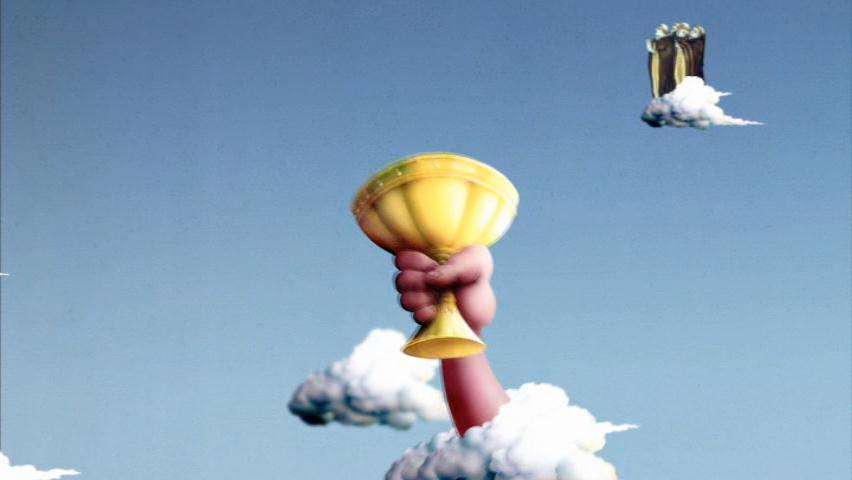
\includegraphics[width=0.8\textwidth]{grail.jpg}
%   \caption[Voorbeeld figuur.]{\label{fig:grail}Voorbeeld van invoegen van een figuur. Zorg altijd voor een uitgebreid bijschrift dat de figuur volledig beschrijft zonder in de tekst te moeten gaan zoeken. Vergeet ook je bronvermelding niet!}
% \end{figure}

% \begin{listing}
%   \begin{minted}{python}
%     import pandas as pd
%     import seaborn as sns

%     penguins = sns.load_dataset('penguins')
%     sns.relplot(data=penguins, x="flipper_length_mm", y="bill_length_mm", hue="species")
%   \end{minted}
%   \caption[Voorbeeld codefragment]{Voorbeeld van het invoegen van een codefragment.}
% \end{listing}

% \lipsum[7-20]

% \begin{table}
%   \centering
%   \begin{tabular}{lcr}
%     \toprule
%     \textbf{Kolom 1} & \textbf{Kolom 2} & \textbf{Kolom 3} \\
%     $\alpha$         & $\beta$          & $\gamma$         \\
%     \midrule
%     A                & 10.230           & a                \\
%     B                & 45.678           & b                \\
%     C                & 99.987           & c                \\
%     \bottomrule
%   \end{tabular}
%   \caption[Voorbeeld tabel]{\label{tab:example}Voorbeeld van een tabel.}
% \end{table}

Als modern IT bedrijf is het belangrijk om de veiligheid van de data te garanderen. Dit is een van de redenen waarom het bedrijf heeft gekozen voor een Zero Trust Netwerkarchitectuur. 
Deze studie onderzoekt de implementatie van een Zero Trust Netwerkarchitectuur en een least privileged access model binnen de hybride cloudomgeving van een softwarebedrijf gebruikmakend van het netskope platform.
Als eerste stap in dit onderzoek is het belangrijk om de huidige situatie van het bedrijf te analyseren. Dit omvat een overzicht van de huidige security-risico’s en tekortkomingen in de huidige perimeterbeveiliging.
Dit wordt gedaan door een analyse van de huidige infrastructuur en de security-risico’s die hiermee gepaard gaan. Alsook door interviews met de IT-afdeling en de security-afdeling van het bedrijf.

Zero Trust is een steeds belangrijker wordend model voor netwerkbeveiliging, vooral in omgevingen waar gevoelige data verwerkt wordt. 
Het model is gebaseerd op de stelling dat geen enkel apparaat, gebruiker of systeem automatisch te vertrouwen is, zelfs niet als deze zich binnen het netwerk bevinden. 
De nadruk ligt op het continu verifiëren van gebruikersidentiteit, het beperken van toegang tot strikt noodzakelijke bronnen (least privileged access), en het monitoren van netwerkactiviteiten om verdachte handelingen snel te identificeren en aan te pakken.

Netskope, het platform dat het bedrijf heeft gekozen voor hun Zero Trust implementatie, definieert Zero Trust als een beveiligingsmodel waarbij niemand blind vertrouwd wordt binnen het netwerk of toegang krijgt tot resources, applicaties of data totdat ze gevalideerd zijn als legitieme gebruiker met een legitieme behoefte~\autocite{Netskope2020}. Hun Security Service Edge (SSE) architectuur implementeert deze principes via een data-centrische aanpak gebaseerd op zes kernpijlers:

\begin{itemize}
  \item User \& Device: Authenticatie en autorisatie van gebruikers en apparaten
  \item Network \& Environment: Segmentatie en toegangscontrole op netwerkniveau
  \item Application \& Workload: Applicatie-specifieke toegangscontrole en monitoring
  \item Data: Databescherming en classificatie
  \item Visibility \& Analytics: Continue monitoring en gedragsanalyse
  \item Automation \& Orchestration: Geautomatiseerde response en integratie
\end{itemize}

Volgens Microsoft is de kern van het Zero Trust-model gebaseerd op drie belangrijke principes: altijd verifiëren, nooit vertrouwen; minimaal toegang verlenen; en schade beperken bij inbreuk. Dit houdt in dat de toegang tot systemen of data niet alleen wordt beperkt op basis van de locatie van de gebruiker of het apparaat, maar altijd afhangt van de identiteit, rol en andere specifieke toegangsbeperkingen~\autocite{Microsoft2024}. Netskope implementeert deze principes via een gelaagde aanpak met Policy Enforcement Points (PEPs) op drie niveaus:

\begin{itemize}
  \item Network/Resource PEP: Controleert netwerktoegang en basiscommunicatie
  \item Application PEP: Beheert toegang tot specifieke applicaties en workloads
  \item Data PEP: Zorgt voor databescherming en compliance
\end{itemize}

Kaspersky benadrukt het belang van de technologieën die Zero Trust mogelijk maken, zoals multi-factor authenticatie (MFA), versleuteling van communicatie en geavanceerde netwerkmonitoringtools~\autocite{Kaspersky2024}. Netskope's platform integreert deze technologieën in een uitgebreid security framework dat onder andere bestaat uit:

\begin{itemize}
  \item Device en user authenticatie via een client certificaat infrastructuur
  \item TLS-beveiligde tunneling voor alle communicatie
  \item Data Loss Prevention (DLP) met meer dan 3000 data identifiers en 1400 bestandstypes
  \item Machine learning-gebaseerde User and Entity Behavior Analytics (UEBA)
  \item Real-time threat protection met meer dan 40 threat intelligence feeds
\end{itemize}

De implementatie van Zero Trust vereist zorgvuldige planning, vooral in complexe netwerkomgevingen.

Uit onderzoek van MIT Lincoln Laboratory blijkt dat Zero Trust-architecturen bijzonder effectief zijn tegen insiderdreigingen, zoals misbruik van gecompromitteerde credentials of onbevoegde toegang door eigen medewerkers. 
Dit risico is relevant voor het onderzochte bedrijf, waar ontwikkelaars en externe partners toegang hebben tot gevoelige klantdata. 
MIT benadrukt dat een succesvolle Zero Trust-implementatie niet alleen technologische verandering vereist (zoals granular access control), maar ook organisatorische aanpassingen, zoals het trainen van medewerkers en het opstellen van duidelijk beleid voor toegangsverificatie. 
Dit sluit aan bij Netskope’s focus op User \& Device workflows en gedragsanalyse, waarbij continue verificatie van gebruikers en apparaten centraal staat. 
Tegelijkertijd waarschuwt MIT voor de complexiteit van hybride implementaties, waarbij on-premises systemen en clouddiensten geïntegreerd moeten worden—een uitdaging die het bedrijf direct ondervindt en waar Netskope’s SSE-platform een antwoord op biedt.~\autocite{MIT2022}

Netskope biedt hiervoor een gestructureerde aanpak met specifieke operationele workflows:

\begin{itemize}
  \item User/Device workflow voor initiële authenticatie en continue validatie
  \item Network/Resource workflow voor toegangscontrole en segmentatie
  \item Data Protection workflow voor databescherming en compliance
\end{itemize}

Deze workflows worden ondersteund door een automation engine die continue monitoring uitvoert op zeven dimensies van gebruikersactiviteit: tijd, dag, locatie, apparaat, service, activiteit en object. Dit zorgt voor een dynamische beveiligingsposture die zich aanpast aan veranderende omstandigheden en dreigingen~\autocite{Netskope2020}.

Het onderzoek van Mutemwa et al. levert een belangrijke bijdrage aan ons begrip van de veranderende aard van cybersecurity in een post-pandemische wereld. Hun studie bevestigt dat traditionele perimeterbescherming fundamenteel is uitgedaagd door de verschuiving naar gedistribueerde werkomgevingen.
De auteurs concluderen dat organisaties moeten evolueren van een perimeter-gebaseerd beveiligingsmodel naar een meer holistische benadering die rekening houdt met de realiteit van een uitgebreide, poreuze bedrijfsgrens. Dit vereist een heroverweging van beveiligingsarchitecturen, met grotere nadruk op identiteitsbeheer, endpoint-beveiliging en gebruikerseducatie.
Deze studie onderstreept de noodzaak voor organisaties om hun cybersecurity-strategieën aan te passen aan een wereld waarin de traditionele grenzen tussen “binnen” en “buiten” het bedrijfsnetwerk steeds vager worden, een conclusie die aansluit bij de bredere verschuiving in de richting van zero-trust beveiligingsmodellen in de cybersecurity-gemeenschap~\autocite{ACM2021}.
%%=============================================================================
%% Methodologie
%%=============================================================================

\chapter{\IfLanguageName{dutch}{Methodologie}{Methodology}}%
\label{ch:methodologie}

%% TODO: In dit hoofstuk geef je een korte toelichting over hoe je te werk bent
%% gegaan. Verdeel je onderzoek in grote fasen, en licht in elke fase toe wat
%% de doelstelling was, welke deliverables daar uit gekomen zijn, en welke
%% onderzoeksmethoden je daarbij toegepast hebt. Verantwoord waarom je
%% op deze manier te werk gegaan bent.
%% 
%% Voorbeelden van zulke fasen zijn: literatuurstudie, opstellen van een
%% requirements-analyse, opstellen long-list (bij vergelijkende studie),
%% selectie van geschikte tools (bij vergelijkende studie, "short-list"),
%% opzetten testopstelling/PoC, uitvoeren testen en verzamelen
%% van resultaten, analyse van resultaten, ...
%%
%% !!!!! LET OP !!!!!
%%
%% Het is uitdrukkelijk NIET de bedoeling dat je het grootste deel van de corpus
%% van je bachelorproef in dit hoofstuk verwerkt! Dit hoofdstuk is eerder een
%% kort overzicht van je plan van aanpak.
%%
%% Maak voor elke fase (behalve het literatuuronderzoek) een NIEUW HOOFDSTUK aan
%% en geef het een gepaste titel.

Dit onderzoek volgt een systematische aanpak die bestaat uit drie hoofdfasen: literatuuronderzoek, technische analyse en proof of concept ontwikkeling. De totale onderzoeksduur bedraagt 14 weken.

\section{Fase 1: Literatuuronderzoek (4 weken)}
Fase 1 van het project betreft een literatuuronderzoek van drie weken waarin de technische documentatie van de Netskope architectuur wordt bestudeerd. 

\vspace{2ex}

Ook externe bronnen worden bestudeerd om een beter beeld te krijgen van de SASE architectuur en de verschillende implementaties.

\section{Fase 2: Requirements analyse (1 week)}
Interviews met Team IT om de huidige situatie te analyseren, dit zal een beter inzicht geven in de huidige security risico's en de vereisten voor een Zero Trust implementatie. 
Via deze gesprekken willen we eerst begrijpen hoe het huidige netwerk is opgebouwd, inclusief hoe de verbindingen tussen kantooromgeving en cloudplatformen verlopen. We bekijken welke beveiligingsmaatregelen al aanwezig zijn en hoe goed deze werken. Ook brengen we in kaart welke beveiligingsrisico’s er zijn, vooral op het gebied van toegangsbeheer, gebruikersverificatie en gegevensbescherming.

\vspace{2ex}

Naast de interviews bekijken we ook bestaande documentatie zoals netwerktekeningen, beveiligingsbeleid en rapporten van vroegere incidenten. Door deze combinatie krijgen we een completer beeld. 

\vspace{2ex}

We letten vooral op risico’s die ontstaan door de traditionele “perimeter-gebaseerde” beveiliging, en hoe een Zero Trust aanpak binnen SASE hier verbetering in kan brengen. 

\vspace{2ex}

Deliverable: een oplijsting van de requirements en een overzicht van de huidige situatie.

\section{Fase 3: Proof of concept ontwikkeling (7 weken)}
De volgende zeven weken zijn voorzien voor de daadwerkelijke ontwikkeling van het
proof of concept. Hierbij wordt gebruik gemaakt van geschikte tools en technologieën die zijn gevonden tijdens de literatuurstudie en ontwerpfase.

\vspace{2ex}

De PoC zal aan de onderzochte requirements voldoen en zal het onderzochte probleem oplossen. 

\vspace{2ex}

De deliverable is een functioneel proof of concept van het netskope systeem.

\section{Fase 4: Validatie en evaluatie (2 weken)}
De ontwikkelde proof of concept wordt geëvalueerd en gevalideerd. Deze fase omvat testen van de functionaliteit, prestaties en
feedback van gebruikers. Eventuele aanpassingen worden doorgevoerd. 

\vspace{2ex}

De einddeliverable omvat een afgewerkt proof of concept.

\vspace{4ex}

Deze methodologie is specifiek afgestemd op de implementatie van een SASE architectuur via het Netskope platform, waarbij elke fase concrete technische deliverables oplevert. De focus ligt op het correct configureren en valideren van Netskope's security features, met voldoende tijd voor iteratie en optimalisatie van de implementatie.



% Voeg hier je eigen hoofdstukken toe die de ``corpus'' van je bachelorproef
% vormen. De structuur en titels hangen af van je eigen onderzoek. Je kan bv.
% elke fase in je onderzoek in een apart hoofdstuk bespreken.

%\input{...}
%\input{...}
%...

%%=============================================================================
%% Conclusie
%%=============================================================================

\chapter{Conclusie}%
\label{ch:conclusie}

% TODO: Trek een duidelijke conclusie, in de vorm van een antwoord op de
% onderzoeksvra(a)g(en). Wat was jouw bijdrage aan het onderzoeksdomein en
% hoe biedt dit meerwaarde aan het vakgebied/doelgroep? 
% Reflecteer kritisch over het resultaat. In Engelse teksten wordt deze sectie
% ``Discussion'' genoemd. Had je deze uitkomst verwacht? Zijn er zaken die nog
% niet duidelijk zijn?
% Heeft het onderzoek geleid tot nieuwe vragen die uitnodigen tot verder 
%onderzoek?

\section{Beantwoording van de onderzoeksvraag}

De centrale onderzoeksvraag "Hoe kan een SASE-architectuur worden geïmplementeerd binnen de hybride cloudomgeving van een softwarebedrijf gebruikmakend van het Netskope platform?" kan op basis van dit onderzoek en de gemeten resultaten positief worden beantwoord. Het ontwikkelde proof of concept toont concrete en meetbare resultaten die de effectiviteit van de SASE-implementatie valideren.

\vspace{2ex}

De implementatie heeft aangetoond dat de geïdentificeerde netwerk- en security-uitdagingen in de hybride cloudomgeving effectief kunnen worden aangepakt. De traditionele perimetergebaseerde beveiligingsaanpak, die onvoldoende veiligheid en flexibiliteit bood, is vervangen door een Zero Trust-model dat contextbewuste beveiliging realiseert ongeacht gebruikerslocatie of apparaattype. De intelligente traffic steering op basis van gebruikerslocatie, gecombineerd met Okta-integratie voor identiteitsbeheer, zorgt voor een optimale balans tussen beveiliging, gebruikerservaring en prestaties.

\section{Bijdrage aan het onderzoeksdomein}

Dit onderzoek levert een concrete bijdrage aan het domein van SASE-implementaties door het ontwikkelen van een praktische implementatiemethodologie specifiek voor software agency bedrijven. De vierfasenaanpak, literatuuronderzoek, requirements analyse, proof of concept ontwikkeling en validatie, biedt een herhaalbaar framework voor vergelijkbare implementaties.

\section{Meerwaarde voor het vakgebied en doelgroep}

Voor IT-professionals en bedrijven biedt dit onderzoek directe meerwaarde, door het demonstreren van een schaalbare beveiligingsarchitectuur die voldoet aan moderne compliance-eisen zonder de operationele flexibiliteit te beperken. De proof of concept toont aan dat SASE-implementaties niet alleen theoretisch haalbaar zijn, maar ook praktisch realiseerbaar binnen bestaande infrastructuren.

\vspace{2ex}

De integratie met populaire enterprise-tools zoals Okta voor identiteitsbeheer en Jamf voor device management illustreert hoe SASE naadloos kan worden geïntegreerd in bestaande IT-ecosystemen. Dit vermindert de implementatierisico's en verlaagt de drempel voor adoptie door andere organisaties in de sector.

\section{Kritische reflectie op het resultaat}

De resultaten die in Hoofdstuk \ref{ch:resultaten} worden samengevat, waren grotendeels conform de verwachtingen, hoewel enkele aspecten positiever uitvielen dan initieel voorzien. 

\vspace{2ex}

De gebruikersacceptatie van de Netskope Client bleek lager dan verwacht, desondanks de transparante communicatiestrategie en de minimale impact op de dagelijkse workflow. 

\vspace{2ex}

De intelligente traffic steering functionaliteit presteerde beter dan geanticipeerd, met nauwelijks merkbare latentieverschillen voor eindgebruikers. Toch waren de eindgebruikers aanvankelijk terughoudend om de nieuwe client te accepteren, wat wijst op de noodzaak van voortdurende change management inspanningen en training.

\vspace{2ex}

Een positief resultaat was de rijkdom aan analytische gegevens die het Netskope platform genereert. Het Advanced Analytics dashboard biedt inzichten die verder gaan dan louter beveiligingsmonitoring en ook waardevolle business intelligence leveren over applicatiegebruik en gebruikersgedrag.

\vspace{2ex}

Een onverwacht technisch probleem was de SSL certificaat interferentie met CLI tools, waarbij applicaties Netskope's SSL Inspection functionaliteit interpreteerden als potentiële Man-in-the-Middle attacks. Dit probleem werd succesvol opgelost door application-specific bypasses en selective SSL inspection policies, maar onderstreept het belang van uitgebreide applicatie-inventarisatie.

\section{Beperkingen en vervolgonderzoek}

Een belangrijke beperking van dit onderzoek is de beperkte onderzoeksperiode van 14 weken, wat de mogelijkheid om langetermijneffecten en gebruikersadoptie over meerdere maanden te evalueren niet mogelijk maakt. Een langdurig onderzoek zou meer inzicht kunnen geven in de evolutie van gebruikersgedrag en de optimalisatie van security policies over tijd.

\section{Conclusie}

Deze bachelorproef demonstreert dat SASE-architectuur via Netskope een praktisch haalbare oplossing biedt voor moderne hybride cloudomgevingen. De combinatie van company-wide Private Access implementatie (122 apparaten under management) met een testgroep van SWG/CASB functionaliteiten toont een effectieve implementatiestrategie die risico's mitigeert terwijl schaalbaarheid wordt gevalideerd.

\vspace{2ex}

De gemeten resultaten van 3 geblokkeerde malicious sites tot 2.100+ AI-events bij ChatGPT, illustreren niet alleen traditionele beveiligingsvoordelen, maar genereren ook unexpected business intelligence die verder gaat dan conventionele security monitoring. Deze concrete cijfers en inzichten vormen een solide basis voor de aanbeveling tot volledige productie-implementatie van alle SASE-componenten binnen software agency bedrijven.

\section{Onverwachte uitdagingen}
\subsection{Eindgebruikers}
Een van de grootste uitdagingen die ik niet had voorzien was het change management-aspect van de implementatie. Technisch gezien verliep de configuratie van Netskope vrij vlot, maar het overtuigen van eindgebruikers van de voordelen en het wegnemen van privacy-zorgen bleek veel complexer dan verwacht. Dit heeft mij geleerd dat succesvolle IT-implementaties evenveel over menselijke factoren gaan als over technologische.

\subsection{SSL certificaat}
Tijdens de implementatie van de Netskope SASE-architectuur ontstond een onverwacht technisch probleem waarbij verschillende applicaties, voornamelijk Command Line Interface (CLI) tools, faalden in hun normale werking. Deze applicaties genereerden SSL/TLS-gerelateerde fouten en weigerden verbindingen tot stand te brengen met externe services.

\vspace{2ex}

Het probleem werd veroorzaakt door Netskope's SSL Inspection functionaliteit, waarbij de Netskope Client een eigen SSL certificaat plaatst op uitgaande HTTPS-pakketten als onderdeel van de Next Gen Secure Web Gateway (SWG) inspectie. Deze techniek, bekend als SSL decryption, stelt de SASE-oplossing in staat om versleuteld verkeer te inspecteren op malware, data loss prevention (DLP) violations, en policy enforcement.

\vspace{2ex}

CLI tools en verschillende enterprise applicaties interpreteren deze certificaat-substitutie als een potentiële Man-in-the-Middle (MiTM) attack, wat resulteert in:

\begin{itemize}
    \item \textbf{Certificate Pinning violations}: Applicaties die specifieke certificaten verwachten van bekende services
    \item \textbf{Trust store conflicts}: Tools die hun eigen certificaat stores hanteren en geen system-wide certificaat updates accepteren
    \item \textbf{API connectivity failures}: RESTful API clients die strikte SSL verificatie hanteren
    \item \textbf{Package managers}: Tools zoals npm, pip, en apt die beveiligde repositories benaderen
\end{itemize}

\section{Persoonlijke reflectie}
\subsection{Leercurve}
Dit onderzoek heeft mijn begrip van moderne netwerkbeveiliging compleet veranderd. Toen ik begon met dit project, was mijn kennis van Zero Trust en SASE-architecturen grotendeels onbestaand. Het praktisch implementeren van een volledige Netskope-omgeving heeft mij echter doen inzien hoe complex en veelomvattend deze transformatie werkelijk is. De overgang van perimetergebaseerde beveiliging naar een Zero Trust-model vereist niet alleen technische aanpassingen, maar vraagt ook om een complete herziening van hoe organisaties over beveiliging denken. Het vraagt ook een enorme inspanning om de werknemers achter de nieuwe technologie te krijgen, dit was een van de grootste uitdagingen die ik tegenkwam die ik niet had verwacht. Het heeft mij ook een eerste ervaring gegeven met een groot project in een bedrijfsomgeving, wat een waardevolle aanvulling is op mijn academische kennis.


%---------- Bijlagen -----------------------------------------------------------

\appendix

\chapter{Onderzoeksvoorstel}

Het onderwerp van deze bachelorproef is gebaseerd op een onderzoeksvoorstel dat vooraf werd beoordeeld door de promotor. Dat voorstel is opgenomen in deze bijlage.

%% TODO: 
%\section*{Samenvatting}

% Kopieer en plak hier de samenvatting (abstract) van je onderzoeksvoorstel.

% Verwijzing naar het bestand met de inhoud van het onderzoeksvoorstel
%---------- Inleiding ---------------------------------------------------------

% TODO: Is dit voorstel gebaseerd op een paper van Research Methods die je
% vorig jaar hebt ingediend? Heb je daarbij eventueel samengewerkt met een
% andere student?
% Zo ja, haal dan de tekst hieronder uit commentaar en pas aan.

%\paragraph{Opmerking}

% Dit voorstel is gebaseerd op het onderzoeksvoorstel dat werd geschreven in het
% kader van het vak Research Methods dat ik (vorig/dit) academiejaar heb
% uitgewerkt (met medesturent VOORNAAM NAAM als mede-auteur).
% 

\section{Inleiding}%
\label{sec:inleiding}

De IT-sector wordt steeds vaker geconfronteerd met complexe beveiligingsuitdagingen, ook in hybride cloudomgevingen. 
Traditionele netwerkbeveiligingsmodellen, die vertrouwen op perimeterbescherming (waarbij de beveiliging zich vooral richt op het bewaken van de netwerkgrenzen via firewalls en VPNs), zijn niet langer toereikend in een tijdperk waarin remote werken, multi-cloud gebruik en gevoelige data-uitwisseling standaard zijn. 
Zero Trust is een beveiligingsstrategie die steeds meer aandacht krijgt, omdat het uitgaat van het principe "never trust, always verify", en de toegang tot resources strikt beperkt op basis van identiteit en context.

Een software agency bedrijf gespecialiseerd in digitale producten, heeft gekozen voor Netskope als oplossing om een Zero Trust Netwerkarchitectuur en een least privileged access model te implementeren. 
Deze keuze voor Netskope als Security Service Edge (SSE) platform dient niet alleen om gevoelige klantendata beter te beschermen, maar ook om te voldoen aan moderne IT-veiligheidsstandaarden die passen bij hun rol als innovatief technologiebedrijf.
De primaire doelgroep van deze bachelorproef is het interne sysops-team van het bedrijf, dat verantwoordelijk is voor de infrastructuur en beveiliging van hun IT-systemen. 
Secundair is het onderzoek relevant voor IT-professionals die verantwoordelijk zijn voor de implementatie van Zero Trust in vergelijkbare omgevingen.

Hoewel het bedrijf geen acuut beveiligingsprobleem ervaart, willen zij anticiperen op toekomstige risico's en voldoen aan de best practices voor IT-beveiliging.
De vraag die centraal staat in dit onderzoek is: "Hoe kan een Zero Trust Netwerkarchitectuur en een least privileged access model worden geïmplementeerd binnen de hybride cloudomgeving van een software agency bedrijf gebruikmakend van het Netskope platform?"

Om deze hoofdvraag te beantwoorden, wordt het onderzoek opgedeeld in volgende deelvragen:
Probleemdomein:
\begin{itemize}
  \item Welke security-risico's bestaan er in de huidige IT-infrastructuur van het bedrijf die met Netskope's Zero Trust features aangepakt kunnen worden?
  \item Welke security gaps bestaan er in de huidige perimeter-based beveiliging die Netskope moet oplossen?
  \item Hoe verhouden de huidige beveiligingsmaatregelen zich tot de mogelijkheden die Netskope biedt?
\end{itemize}

Oplossingsdomein:
\begin{itemize}
  \item Welke Netskope componenten zijn essentieel voor een succesvolle Zero Trust implementatie?
  \item Hoe kan Netskope optimaal geconfigureerd worden voor de hybride cloudomgeving van het bedrijf?
  \item Hoe kan een least privileged access model worden geïmplementeerd via Netskope's policy engine?
  \item Welke integraties tussen Netskope en bestaande systemen zijn nodig?
  \item Hoe kan de effectiviteit van de Netskope implementatie worden gevalideerd?
\end{itemize}

Het doel van deze bachelorproef is om een praktische invulling te geven aan Zero Trust binnen een software agency bedrijf. Om deze deelvragen te beantwoorden richt het onderzoek zich op drie hoofdaspecten:
\begin{itemize}
  \item Een grondige analyse van de huidige IT-omgeving bij het bedrijf en de bijhorende security-risico's.
  \item Het identificeren van essentiële Netskope componenten en configuraties die aansluiten bij de specifieke context van het bedrijf.
  \item Het ontwerpen en implementeren van een proof of concept die dient als blauwdruk voor toekomstige implementaties.
\end{itemize}

Een succesvol resultaat wordt behaald als er een concreet PoC wordt opgeleverd dat technisch functioneel is en aansluit bij de behoeften van het bedrijf, samen met een rapport waarin aanbevelingen worden gedaan voor de schaalbare implementatie van Zero Trust met Netskope.

%---------- Stand van zaken ---------------------------------------------------
% Hier beschrijf je de \emph{state-of-the-art} rondom je gekozen onderzoeksdomein, d.w.z.\ een inleidende, doorlopende tekst over het onderzoeksdomein van je bachelorproef. Je steunt daarbij heel sterk op de professionele \emph{vakliteratuur}, en niet zozeer op populariserende teksten voor een breed publiek. Wat is de huidige stand van zaken in dit domein, en wat zijn nog eventuele open vragen (die misschien de aanleiding waren tot je onderzoeksvraag!)?

% Je mag de titel van deze sectie ook aanpassen (literatuurstudie, stand van zaken, enz.). Zijn er al gelijkaardige onderzoeken gevoerd? Wat concluderen ze? Wat is het verschil met jouw onderzoek?

% Verwijs bij elke introductie van een term of bewering over het domein naar de vakliteratuur, bijvoorbeeld~\autocite{Hykes2013}! Denk zeker goed na welke werken je refereert en waarom.

%Draag zorg voor correcte literatuurverwijzingen! Een bronvermelding hoort thuis \emph{binnen} de zin waar je je op die bron baseert, dus niet er buiten! Maak meteen een verwijzing als je gebruik maakt van een bron. Doe dit dus \emph{niet} aan het einde van een lange paragraaf. Baseer nooit teveel aansluitende tekst op eenzelfde bron.

% Als je informatie over bronnen verzamelt in JabRef, zorg er dan voor dat alle nodige info aanwezig is om de bron terug te vinden (zoals uitvoerig besproken in de lessen Research Methods).

\section{Literatuurstudie}%
\label{sec:literatuurstudie}

Zero Trust is een steeds belangrijker wordend model voor netwerkbeveiliging, vooral in omgevingen waar gevoelige data verwerkt wordt. 
Het model is gebaseerd op de stelling dat geen enkel apparaat, gebruiker of systeem automatisch te vertrouwen is, zelfs niet als deze zich binnen het netwerk bevinden. 
De nadruk ligt op het continu verifiëren van gebruikersidentiteit, het beperken van toegang tot strikt noodzakelijke bronnen (least privileged access), en het monitoren van netwerkactiviteiten om verdachte handelingen snel te identificeren en aan te pakken.

Netskope, het platform dat het bedrijf heeft gekozen voor hun Zero Trust implementatie, definieert Zero Trust als een beveiligingsmodel waarbij niemand blind vertrouwd wordt binnen het netwerk of toegang krijgt tot resources, applicaties of data totdat ze gevalideerd zijn als legitieme gebruiker met een legitieme behoefte~\autocite{Netskope2020}. Hun Security Service Edge (SSE) architectuur implementeert deze principes via een data-centrische aanpak gebaseerd op zes kernpijlers:

\begin{itemize}
  \item User \& Device: Authenticatie en autorisatie van gebruikers en apparaten
  \item Network \& Environment: Segmentatie en toegangscontrole op netwerkniveau
  \item Application \& Workload: Applicatie-specifieke toegangscontrole en monitoring
  \item Data: Databescherming en classificatie
  \item Visibility \& Analytics: Continue monitoring en gedragsanalyse
  \item Automation \& Orchestration: Geautomatiseerde response en integratie
\end{itemize}

Volgens Microsoft is de kern van het Zero Trust-model gebaseerd op drie belangrijke principes: altijd verifiëren, nooit vertrouwen; minimaal toegang verlenen; en schade beperken bij inbreuk. Dit houdt in dat de toegang tot systemen of data niet alleen wordt beperkt op basis van de locatie van de gebruiker of het apparaat, maar altijd afhangt van de identiteit, rol en andere specifieke toegangsbeperkingen~\autocite{Microsoft2024}. Netskope implementeert deze principes via een gelaagde aanpak met Policy Enforcement Points (PEPs) op drie niveaus:

\begin{itemize}
  \item Network/Resource PEP: Controleert netwerktoegang en basiscommunicatie
  \item Application PEP: Beheert toegang tot specifieke applicaties en workloads
  \item Data PEP: Zorgt voor databescherming en compliance
\end{itemize}

Kaspersky benadrukt het belang van de technologieën die Zero Trust mogelijk maken, zoals multi-factor authenticatie (MFA), versleuteling van communicatie en geavanceerde netwerkmonitoringtools~\autocite{Kaspersky2024}. Netskope's platform integreert deze technologieën in een uitgebreid security framework dat onder andere bestaat uit:

\begin{itemize}
  \item Device en user authenticatie via een client certificaat infrastructuur
  \item TLS-beveiligde tunneling voor alle communicatie
  \item Data Loss Prevention (DLP) met meer dan 3000 data identifiers en 1400 bestandstypes
  \item Machine learning-gebaseerde User and Entity Behavior Analytics (UEBA)
  \item Real-time threat protection met meer dan 40 threat intelligence feeds
\end{itemize}

De implementatie van Zero Trust vereist zorgvuldige planning, vooral in complexe netwerkomgevingen.

Uit onderzoek van MIT Lincoln Laboratory blijkt dat Zero Trust-architecturen bijzonder effectief zijn tegen insiderdreigingen, zoals misbruik van gecompromitteerde credentials of onbevoegde toegang door eigen medewerkers. 
Dit risico is relevant voor het onderzochte bedrijf, waar ontwikkelaars en externe partners toegang hebben tot gevoelige klantdata. 
MIT benadrukt dat een succesvolle Zero Trust-implementatie niet alleen technologische verandering vereist (zoals granular access control), maar ook organisatorische aanpassingen, zoals het trainen van medewerkers en het opstellen van duidelijk beleid voor toegangsverificatie. 
Dit sluit aan bij Netskope’s focus op User \& Device workflows en gedragsanalyse, waarbij continue verificatie van gebruikers en apparaten centraal staat. 
Tegelijkertijd waarschuwt MIT voor de complexiteit van hybride implementaties, waarbij on-premises systemen en clouddiensten geïntegreerd moeten worden—een uitdaging die het bedrijf direct ondervindt en waar Netskope’s SSE-platform een antwoord op biedt.~\autocite{MIT2022}

Netskope biedt hiervoor een gestructureerde aanpak met specifieke operationele workflows:

\begin{itemize}
  \item User/Device workflow voor initiële authenticatie en continue validatie
  \item Network/Resource workflow voor toegangscontrole en segmentatie
  \item Data Protection workflow voor databescherming en compliance
\end{itemize}

Deze workflows worden ondersteund door een automation engine die continue monitoring uitvoert op zeven dimensies van gebruikersactiviteit: tijd, dag, locatie, apparaat, service, activiteit en object. Dit zorgt voor een dynamische beveiligingsposture die zich aanpast aan veranderende omstandigheden en dreigingen~\autocite{Netskope2020}.

Deze literatuurstudie toont aan dat de keuze van het bedrijf voor Netskope aansluit bij moderne best practices voor Zero Trust implementatie. Het platform biedt niet alleen de technische capabilities voor robuuste beveiliging, maar ook de flexibiliteit en schaalbaarheid die nodig zijn voor een hybride cloudomgeving. De gelaagde aanpak met specifieke PEPs en geautomatiseerde workflows zorgt voor een balans tussen strikte beveiliging en operationele efficiëntie.
% Voor literatuurverwijzingen zijn er twee belangrijke commando's:
% \autocite{KEY} => (Auteur, jaartal) Gebruik dit als de naam van de auteur
%   geen onderdeel is van de zin.
% \textcite{KEY} => Auteur (jaartal)  Gebruik dit als de auteursnaam wel een
%   functie heeft in de zin (bv. ``Uit onderzoek door Doll & Hill (1954) bleek
%   ...'')

% Je mag deze sectie nog verder onderverdelen in subsecties als dit de structuur van de tekst kan verduidelijken.

%---------- Methodologie ------------------------------------------------------
% Hier beschrijf je hoe je van plan bent het onderzoek te voeren. Welke onderzoekstechniek ga je toepassen om elk van je onderzoeksvragen te beantwoorden? Gebruik je hiervoor literatuurstudie, interviews met belanghebbenden (bv.~voor requirements-analyse), experimenten, simulaties, vergelijkende studie, risico-analyse, PoC, \ldots?

%Valt je onderwerp onder één van de typische soorten bachelorproeven die besproken zijn in de lessen Research Methods (bv.\ vergelijkende studie of risico-analyse)? Zorg er dan ook voor dat we duidelijk de verschillende stappen terug vinden die we verwachten in dit soort onderzoek!

%Vermijd onderzoekstechnieken die geen objectieve, meetbare resultaten kunnen opleveren. Enquêtes, bijvoorbeeld, zijn voor een bachelorproef informatica meestal \textbf{niet geschikt}. De antwoorden zijn eerder meningen dan feiten en in de praktijk blijkt het ook bijzonder moeilijk om voldoende respondenten te vinden. Studenten die een enquête willen voeren, hebben meestal ook geen goede definitie van de populatie, waardoor ook niet kan aangetoond worden dat eventuele resultaten representatief zijn.

%Uit dit onderdeel moet duidelijk naar voor komen dat je bachelorproef ook technisch voldoen\-de diepgang zal bevatten. Het zou niet kloppen als een bachelorproef informatica ook door bv.\ een student marketing zou kunnen uitgevoerd worden.

%Je beschrijft ook al welke tools (hardware, software, diensten, \ldots) je denkt hiervoor te gebruiken of te ontwikkelen.

%Probeer ook een tijdschatting te maken. Hoe lang zal je met elke fase van je onderzoek bezig zijn en wat zijn de concrete \emph{deliverables} in elke fase?

\section{Methodologie}%
\label{sec:methodologie}

Dit onderzoek volgt een systematische aanpak die bestaat uit drie hoofdfasen: literatuuronderzoek, technische analyse, en proof of concept ontwikkeling. De totale onderzoeksduur bedraagt 14 weken.

\subsection{Fase 1: Literatuuronderzoek (3 weken)}
Deze fase richt zich op het verzamelen van theoretische kennis en best practices:
\begin{itemize}
  \item Week 1-2: 
  \begin{itemize}
    \item Analyse van Netskope's technische documentatie en architectuur
    \item Bestudering van Netskope's Zero Trust Reference Architecture
    \item Onderzoek naar best practices voor Netskope implementaties
  \end{itemize}
  \item Week 3: 
  \begin{itemize}
    \item Synthese van bevindingen
    \item Opstellen van Netskope-specifiek implementatieplan
  \end{itemize}
  \item Deliverable: Implementatieplan met Netskope configuratierichtlijnen
\end{itemize}

\subsection{Fase 2: Technische analyse (4 weken)}

\subsubsection{Security audit (2 weken)}
\begin{itemize}
  \item Week 1: 
  \begin{itemize}
    \item Analyse van huidige netwerkinfrastructuur voor Netskope integratie
    \item Inventarisatie van te beveiligen resources en applicaties
  \end{itemize}
  \item Week 2:
  \begin{itemize}
    \item Assessment van integratiepunten voor Netskope
    \item Identificatie van benodigde Policy Enforcement Points
  \end{itemize}
  \item Deliverable: Technisch rapport met integratievereisten
\end{itemize}

\subsubsection{Requirements analyse (2 weken)}
\begin{itemize}
  \item Analyse van gebruikersprofielen voor Netskope policies
  \item Identificatie van kritieke applicaties en data flows
  \item In kaart brengen van benodigde security policies
  \item Deliverable: Requirements document voor Netskope configuratie
\end{itemize}

\subsection{Fase 3: Proof of Concept (7 weken)}

\subsubsection{PoC Setup (4 weken)}
Ontwikkeling van testomgeving met Netskope componenten:

\begin{enumerate}
  \item Week 1-2: Basis infrastructuur
  \begin{itemize}
    \item Opzetten Netskope tenant
    \item Configuratie van Identity and Access Management
    \item Implementatie van Netskope client op test endpoints
  \end{itemize}

  \item Week 3-4: Policy en Security configuratie
  \begin{itemize}
    \item Configuratie van Resource, Application en Data PEPs
    \item Implementatie van security policies
    \item Setup van monitoring en logging
  \end{itemize}
  \item Deliverable: Functionele Netskope PoC omgeving
\end{enumerate}

\subsubsection{PoC Validatie (3 weken)}
\begin{itemize}
  \item Week 1: Security testing
  \begin{itemize}
    \item Validatie van Zero Trust policies
    \item Testing van MFA en toegangscontrole
    \item DLP functionaliteit verificatie
    \item Testing van dynamische toegangscontrole (‘trip wires’)
  \end{itemize}
  
  \item Week 2: Performance testing
  \begin{itemize}
    \item Latency metingen van Netskope security cloud
    \item End-user experience validatie
    \item Resource impact analyse
  \end{itemize}
  
  \item Week 3: Documentatie
  \begin{itemize}
    \item Opstellen van implementatiehandleiding
    \item Documenteren van best practices
    \item Voorbereiden eindrapportage
  \end{itemize}
  \item Deliverable: Validatierapport en implementatiedocumentatie
\end{itemize}

Deze methodologie is specifiek afgestemd op de implementatie van Zero Trust via het Netskope platform, waarbij elke fase concrete technische deliverables oplevert. De focus ligt op het correct configureren en valideren van Netskope's security features, met voldoende tijd voor iteratie en optimalisatie van de implementatie.

%---------- Verwachte resultaten ----------------------------------------------
%Hier beschrijf je welke resultaten je verwacht. Als je metingen en simulaties uitvoert, kan je hier al mock-ups maken van de grafieken samen met de verwachte conclusies. Benoem zeker al je assen en de onderdelen van de grafiek die je gaat gebruiken. Dit zorgt ervoor dat je concreet weet welk soort data je moet verzamelen en hoe je die moet meten.

%Wat heeft de doelgroep van je onderzoek aan het resultaat? Op welke manier zorgt jouw bachelorproef voor een meerwaarde?

%Hier beschrijf je wat je verwacht uit je onderzoek, met de motivatie waarom. Het is \textbf{niet} erg indien uit je onderzoek andere resultaten en conclusies vloeien dan dat je hier beschrijft: het is dan juist interessant om te onderzoeken waarom jouw hypothesen niet overeenkomen met de resultaten.

\section{Verwacht resultaat, conclusie}%
\label{sec:verwachte_resultaten}

Het belangrijkste verwachte resultaat is het succesvol opzetten van een Proof of Concept (PoC) die demonstreert hoe Netskope's Zero Trust architectuur effectief kan worden geïmplementeerd binnen de bestaande infrastructuur van het bedrijf. 
De PoC zal bestaan uit een volledig geconfigureerde Netskope omgeving met:

\begin{itemize}
  \item Een werkende Netskope Security Cloud configuratie die:
  \begin{itemize}
    \item Zero Trust principes implementeert via Netskope's Policy Enforcement Points (PEPs)
    \item Authenticatie en autorisatie strikt controleert op netwerk-, applicatie- en dataniveau
    \item Least privileged access afdwingt via granulaire policies
  \end{itemize}
  
  \item Geïmplementeerde Netskope componenten voor:
  \begin{itemize}
    \item Identity en Access Management integratie
    \item Network/Resource security controls
    \item Data Loss Prevention (DLP)
    \item User and Entity Behavior Analytics (UEBA)
  \end{itemize}
\end{itemize}

De concrete deliverables zullen bestaan uit:

\begin{itemize}
  \item Technische documentatie die beschrijft:
  \begin{itemize}
    \item Netskope tenant configuratie
    \item Policy frameworks voor verschillende gebruikersgroepen
    \item Security policy instellingen
    \item Integratie met bestaande systemen
  \end{itemize}

  \item Validatierapport met:
  \begin{itemize}
    \item Security testresultaten
    \item Performance metrics
    \item User experience analyse
    \item Aanbevelingen voor productie-uitrol
  \end{itemize}

  \item Implementatiehandleiding voor:
  \begin{itemize}
    \item Netskope client deployment
    \item Policy configuratie
    \item Monitoring setup
    \item Incident response procedures
  \end{itemize}
\end{itemize}

De belangrijkste meerwaarde voor het bedrijf is een versterkte security posture door:
\begin{itemize}
  \item Centraal beheer van security policies via Netskope's unified platform
  \item Verbeterde zichtbaarheid in gebruikersactiviteit en datastromen
  \item Geautomatiseerde threat detection en response
  \item Schaalbare security architectuur die past bij hun groei
\end{itemize}

De implementatie van Zero Trust via Netskope biedt het bedrijf niet alleen een robuuste beveiligingsarchitectuur, maar ook een strategisch voordeel in een snel veranderende IT-omgeving. 
Door technologische innovatie te combineren met organisatorische aanpassingen, kan het bedrijf haar positie als innovatief technologiebedrijf verder versterken en voldoen aan de hoogste standaarden voor IT-veiligheid. 
De PoC zal dienen als blauwdruk voor de uiteindelijke productie-implementatie van Netskope binnen de organisatie.
Hoewel de PoC binnen een tijdsbestek van 14 weken wordt uitgevoerd, benadrukt onderzoek van MIT Lincoln Laboratory dat volledige Zero Trust-implementaties vaak 3–5 jaar vergen vanwege organisatorische complexiteit, zoals het trainen van medewerkers en het integreren van legacy-systemen.~\autocite{MIT2022}
Dit impliceert dat de PoC vooral dient als eerste stap, waarbij de schaalbaarheid van de voorgestelde oplossing en het langetermijncommitment van het bedrijf essentieel zijn voor een succesvolle productie-uitrol. 
Daarnaast richt deze studie zich specifiek op Netskope, waardoor vergelijkende analyses met andere Zero Trust-platforms (zoals Zscaler of Palo Alto Prisma) buiten beschouwing blijven. 

%%---------- Andere bijlagen --------------------------------------------------
% TODO: Voeg hier eventuele andere bijlagen toe. Bv. als je deze BP voor de
% tweede keer indient, een overzicht van de verbeteringen t.o.v. het origineel.
%\input{...}

%%---------- Backmatter, referentielijst ---------------------------------------

\backmatter{}

\setlength\bibitemsep{2pt} %% Add Some space between the bibliograpy entries
\printbibliography[heading=bibintoc]

\end{document}
